\mbox{$\displaystyle $\,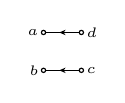
\begin{tikzpicture}[x=0.340cm, y=0.340cm, line width=0.420pt, baseline={([yshift=-0.6ex]0,0)}]
  \draw (0.707,0.707) -- (-0.707,0.707);
  \fill (-0.119,0.707) -- (0.119,0.605) -- (0.042,0.707) -- (0.119,0.809) -- cycle;
  \draw (0.707,-0.707) -- (-0.707,-0.707);
  \fill (-0.119,-0.707) -- (0.119,-0.809) -- (0.042,-0.707) -- (0.119,-0.605) -- cycle;
  \draw[fill=white] (-0.707,0.707) circle (0.080);
  \draw[fill=white] (-0.707,-0.707) circle (0.080);
  \draw[fill=white] (0.707,-0.707) circle (0.080);
  \draw[fill=white] (0.707,0.707) circle (0.080);
  \node[font=\tiny, inner sep=0pt, anchor=0] at (-0.877,0.707) {$a$};
  \node[font=\tiny, inner sep=0pt, anchor=0] at (-0.877,-0.707) {$b$};
  \node[font=\tiny, inner sep=0pt, anchor=180] at (0.877,-0.707) {$c$};
  \node[font=\tiny, inner sep=0pt, anchor=180] at (0.877,0.707) {$d$};
\end{tikzpicture}}
\diagramgap
\mbox{$\displaystyle -\,$\,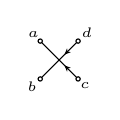
\begin{tikzpicture}[x=0.340cm, y=0.340cm, line width=0.420pt, baseline={([yshift=-0.6ex]0,0)}]
  \draw (0.707,-0.707) -- (-0.707,0.707);
  \fill (0.198,-0.198) -- (0.295,-0.439) -- (0.312,-0.312) -- (0.439,-0.295) -- cycle;
  \draw (0.707,0.707) -- (-0.707,-0.707);
  \fill (0.198,0.198) -- (0.439,0.295) -- (0.312,0.312) -- (0.295,0.439) -- cycle;
  \draw[fill=white] (-0.707,0.707) circle (0.080);
  \draw[fill=white] (-0.707,-0.707) circle (0.080);
  \draw[fill=white] (0.707,-0.707) circle (0.080);
  \draw[fill=white] (0.707,0.707) circle (0.080);
  \node[font=\tiny, inner sep=0pt, anchor=315] at (-0.827,0.827) {$a$};
  \node[font=\tiny, inner sep=0pt, anchor=45] at (-0.827,-0.827) {$b$};
  \node[font=\tiny, inner sep=0pt, anchor=135] at (0.827,-0.827) {$c$};
  \node[font=\tiny, inner sep=0pt, anchor=225] at (0.827,0.827) {$d$};
\end{tikzpicture}}
